\let\negmedspace\undefined
\let\negthickspace\undefined
\documentclass[journal,12pt,onecolumn]{IEEEtran}
\usepackage{cite}
\usepackage{amsmath,amssymb,amsfonts,amsthm}
\usepackage{algorithmic}
\usepackage{graphicx}
\usepackage{textcomp}
\usepackage{xcolor}
\usepackage{txfonts}
\usepackage{listings}
\usepackage{enumitem}
\usepackage{mathtools}
\usepackage{gensymb}
\usepackage[breaklinks=true]{hyperref}
\usepackage{tkz-euclide} % loads  TikZ and tkz-base
\usepackage{listings}
\usepackage{caption}


\newtheorem{theorem}{Theorem}[section]
\newtheorem{problem}{Problem}
\newtheorem{proposition}{Proposition}[section]
\newtheorem{lemma}{Lemma}[section]
\newtheorem{corollary}[theorem]{Corollary}
\newtheorem{example}{Example}[section]
\newtheorem{definition}[problem]{Definition}
%\newtheorem{thm}{Theorem}[section] 
%\newtheorem{defn}[thm]{Definition}
%\newtheorem{algorithm}{Algorithm}[section]
%\newtheorem{cor}{Corollary}
\newcommand{\BEQA}{\begin{eqnarray}}
\newcommand{\EEQA}{\end{eqnarray}}
\newcommand{\define}{\stackrel{\triangle}{=}}
\theoremstyle{remark}
\newtheorem{rem}{Remark}
%\bibliographystyle{ieeetr}
\begin{document}
%
\providecommand{\pr}[1]{\ensuremath{\Pr\left(#1\right)}}
\providecommand{\prt}[2]{\ensuremath{p_{#1}^{\left(#2\right)} }}        % own macro for this question
\providecommand{\qfunc}[1]{\ensuremath{Q\left(#1\right)}}
\providecommand{\sbrak}[1]{\ensuremath{{}\left[#1\right]}}
\providecommand{\lsbrak}[1]{\ensuremath{{}\left[#1\right.}}
\providecommand{\rsbrak}[1]{\ensuremath{{}\left.#1\right]}}
\providecommand{\brak}[1]{\ensuremath{\left(#1\right)}}
\providecommand{\lbrak}[1]{\ensuremath{\left(#1\right.}}
\providecommand{\rbrak}[1]{\ensuremath{\left.#1\right)}}
\providecommand{\cbrak}[1]{\ensuremath{\left\{#1\right\}}}
\providecommand{\lcbrak}[1]{\ensuremath{\left\{#1\right.}}
\providecommand{\rcbrak}[1]{\ensuremath{\left.#1\right\}}}
\newcommand{\sgn}{\mathop{\mathrm{sgn}}}
\providecommand{\abs}[1]{\left\vert#1\right\vert}
\providecommand{\res}[1]{\Res\displaylimits_{#1}} 
\providecommand{\norm}[1]{\left\lVert#1\right\rVert}
%\providecommand{\norm}[1]{\lVert#1\rVert}
\providecommand{\mtx}[1]{\mathbf{#1}}
\providecommand{\mean}[1]{E\left[ #1 \right]}
\providecommand{\cond}[2]{#1\middle|#2}
\providecommand{\fourier}{\overset{\mathcal{F}}{ \rightleftharpoons}}
\newenvironment{amatrix}[1]{%
  \left(\begin{array}{@{}*{#1}{c}|c@{}}
}{%
  \end{array}\right)
}
%\providecommand{\hilbert}{\overset{\mathcal{H}}{ \rightleftharpoons}}
%\providecommand{\system}{\overset{\mathcal{H}}{ \longleftrightarrow}}
	%\newcommand{\solution}[2]{\textbf{Solution:}{#1}}
\newcommand{\solution}{\noindent \textbf{Solution: }}
\newcommand{\cosec}{\,\text{cosec}\,}
\providecommand{\dec}[2]{\ensuremath{\overset{#1}{\underset{#2}{\gtrless}}}}
\newcommand{\myvec}[1]{\ensuremath{\begin{pmatrix}#1\end{pmatrix}}}
\newcommand{\mydet}[1]{\ensuremath{\begin{vmatrix}#1\end{vmatrix}}}
\newcommand{\myaugvec}[2]{\ensuremath{\begin{amatrix}{#1}#2\end{amatrix}}}
\providecommand{\rank}{\text{rank}}
\providecommand{\pr}[1]{\ensuremath{\Pr\left(#1\right)}}
\providecommand{\qfunc}[1]{\ensuremath{Q\left(#1\right)}}
	\newcommand*{\permcomb}[4][0mu]{{{}^{#3}\mkern#1#2_{#4}}}
\newcommand*{\perm}[1][-3mu]{\permcomb[#1]{P}}
\newcommand*{\comb}[1][-1mu]{\permcomb[#1]{C}}
\providecommand{\qfunc}[1]{\ensuremath{Q\left(#1\right)}}
\providecommand{\gauss}[2]{\mathcal{N}\ensuremath{\left(#1,#2\right)}}
\providecommand{\diff}[2]{\ensuremath{\frac{d{#1}}{d{#2}}}}
\providecommand{\myceil}[1]{\left \lceil #1 \right \rceil }
\newcommand\figref{Fig.~\ref}
\newcommand\tabref{Table~\ref}
\newcommand{\sinc}{\,\text{sinc}\,}
\newcommand{\rect}{\,\text{rect}\,}
%%
%	%\newcommand{\solution}[2]{\textbf{Solution:}{#1}}
%\newcommand{\solution}{\noindent \textbf{Solution: }}
%\newcommand{\cosec}{\,\text{cosec}\,}
%\numberwithin{equation}{section}
%\numberwithin{equation}{subsection}
%\numberwithin{problem}{section}
%\numberwithin{definition}{section}
%\makeatletter
%\@addtoreset{figure}{problem}
%\makeatother

%\let\StandardTheFigure\thefigure
\let\vec\mathbf

\bibliographystyle{IEEEtran}


\vspace{3cm}



\bigskip

\renewcommand{\thefigure}{\theenumi}
\renewcommand{\thetable}{\theenumi}
%\renewcommand{\theequation}{\theenumi}
Q:The difference between any two cosecutive interior angles of a polygon is $5^\circ$.If the smallest angle is $120^\circ$,find the number of sides of polygon.
\\\solution
The interior angles of a polygon are in AP with
\begin{align*}
    x(0)&=120\\
    d&=5
\end{align*}
The sum of n terms of an AP is given by
\begin{equation}
    S=\frac{n}{2}(2\cdot x(0)+(n-1)d)
\end{equation}
Sum of interior angles of AP is given by
\begin{equation}
    S=(n-2)180
\end{equation}
\[\frac{n}{2}(2\cdot x(0)+(n-1)d)= (n-2)180 \]
\[
\begin{aligned}
    \frac{n}{2}(240+(n-1)5)&=(n-2)180\\
    n(235+5n)&=360n-720\\
    5n^2+235n&=360n-720\\
    5n^2-125+720&=0\\
    n^2-25n+144&=0
\end{aligned}
\]
solving the above equation we get
\[
\begin{aligned}
   n=16,9
\end{aligned}
\]
\[ x(n) = \begin{cases}
          120 + 5n & \text{if }0 \leq n\leq 15 \\
          0 & \text{if } n >15 , n<0
       \end{cases} \]

\begin{figure}[h]
  \centering
  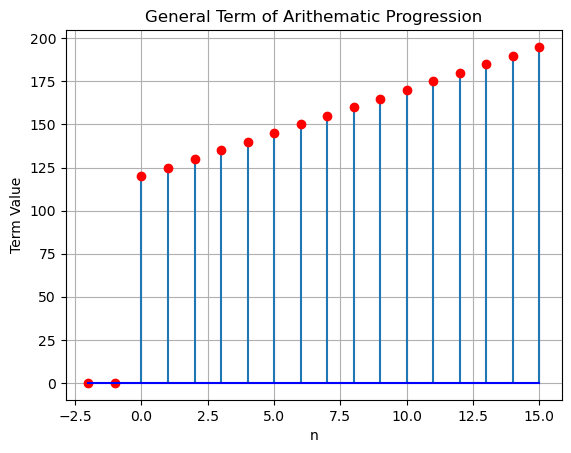
\includegraphics[width=0.5\linewidth]{/home/meena/figs/python.1(1).png} % Replace "path/to/your/image" with the actual file path or URL
  \captionsetup{justification=centering}
  \caption{Plot of the general term taken from Python}
  \label{fig:your_label}
\end{figure}
\[
X(n) = \sum_{n=-\infty}^{\infty} x(n) \cdot z^{-n}\cdot u(n)
\]
The expression for \(X(z)\) is given by:
\[
X(z) = \sum_{n=0}^{15} (120 + 5n) \cdot z^{-n} \cdot u[n]
\]
The above sequence  converges for \(\lvert z \rvert > 15\)\\
The expression for u(n) is 
\[ u(n) = \begin{cases}
    1 & \text{if } n \geq 0, \\
    0 & \text{if } n < 0.
\end{cases} \]
We can evaluate the summation term by term. The unit step function u[n] ensures that only the terms with \(n \geq 0\) are considered.
Evaluating the sum term by term, we get:
\[
\begin{aligned}
X(z) &= 120 \cdot z^0 + (120 + 5 \cdot 1) \cdot z^{-1} + (120 + 5 \cdot 2) \cdot z^{-2} + \ldots + (120 + 5 \cdot 15) \cdot z^{-15} \\
&= 120 + 125 \cdot z^{-1} + 130 \cdot z^{-2} + \ldots + 195 \cdot z^{-15}
\end{aligned}
\]
%\[
%X(n) = \sum_{n=1}^{16} (115+5n) \cdot z^{-n}
%\]
\[
\begin{aligned}
   X(n) = \sum_{n=0}^{15} (120+5n) \cdot z^{-n}\\
   X(n) = 120\sum_{n=0}^{15}z^{-n}+5\sum_{n=0}^{15}n\cdot z^{-n}
\end{aligned}
\]
Let \(p = 120 \cdot \sum_{n=0}^{15} z^{-n}\), \(q = 5\sum_{n=0}^{15}n\cdot z^{-n}\)\\
By using formula of sum of n terms of GP we get
\[\therefore\ p=120\times \frac{ ( z^{-16}-1)}{(z^{-1}-1)}=120\times \frac{ (1 - z^{-16})}{(1 - z^{-1})} \]
\[p=\frac{120-120 z^{-16}}{(1 - z^{-1})}\]
\[
   q= 5\sum_{n=0}^{15}n\cdot z^{-n}
\]
The terms of q are in AGP. Hence the sum is given by


\[
\begin{aligned}
   \sum_{n=0}^{15}n\cdot z^{-n}&= \frac{1}{1 - z^{-1} }+ \frac{z^{-1}(1 - z^{-15})}{(1 - z^{-1})^2}-\frac{(1+(16-1)1)\times z^{-16}}{1-z^{-1}} \\
&=\frac{1}{1 - z^{-1} }+ \frac{z^{-1}(1 - z^{-15})}{(1 - z^{-1})^2}-\frac{16\times z^{-16}}{1-z^{-1}}\\
&=\frac{(1-z^{-1})+(z^{-1}-z^{-16})-16\cdot z^{-16}(1-z^{-1})}{(1-z^{-1})^{2}}\\
&=\frac{(1-z^{-1})+(z^{-1}-z^{-16})-16z^{-16}-z^{-17})}{(1-z^{-1})^{2}}\\
&=\frac{1-z^{-1}+z^{-1}-z^{-16}-16\cdot z^{-16}+16\cdot z^{-17}}{(1-z^{-1})^{2}}\\
&=\frac{1-17\cdot z^{-16}+16\cdot z^{-17}}{(1-z^{-1})^{2}}\\
q&=5\times \sum_{n=1}^{16}n\cdot z^{-(n-1)}\\
\therefore \ q&=\frac{5-85\cdot z^{-16}+80\cdot z^{-17}}{(1-z^{-1})^{2}}
\end{aligned}
\]
\[
\begin{aligned}
   X(n)&=p+q\\
   &=\frac{120 -120 z^{-16}}{1-z^{-1}}+\frac{5-85\cdot z^{-16}+80\cdot z^{-17}}{(1-z^{-1})^{2}}\\
   &=\frac{(120 -120 z^{-16})(1-z^{-1})+(5-85\cdot z^{-16}+80\cdot z^{-17})}{(1-z^{-1})^2}\\
   &=\frac{(120-120 z^{-16}-120 z^{-1}+120\cdot z^{-17})+(5-85\cdot z^{-16}+80\cdot z^{-17})}{(1-z^{-1})^2}\\
\end{aligned}
\]
\begin{equation}
\therefore X(z) = \frac{125 -120 z^{-1}-205 z^{-16}+200 z^{-17}}{(1-z^{-1})^2} u(z) \quad \forall \lvert z \rvert > 15.
\end{equation}
The expression for \( u(z) \) is given by:
\[
u(z) = 
\begin{cases}
    0, & \text{for } z < 0, z \in \mathbb{Z}, \\
    1, & \text{for } z > 0, z \in \mathbb{Z}.
\end{cases}
\]
now the expression simplifies to 
\begin {equation}
X(z) = \frac{125 -120 z^{-1}-205 z^{-16}+200 z^{-17}}{(1-z^{-1})^2} u(z) \quad \forall z>5
\end {equation}
\begin{table}[h]
  \centering
  \begin{tabular}{|c|c|c|}
    \hline
      \textbf{Variable}& \textbf{Description}& \textbf{Value}\\\hline
    x(0)& first term of AP& 120  \\\hline
    d& common difference of AP & 5\\\hline
    x(n) & general  term of AP&none\\\hline
   n & Describing the order of term & none\\\hline
    u(n)& unit step function & mentioned above\\\hline
    u(z) & z-transform of u(n) & mentioned above\\\hline
    X(z)& z-transform of u(n) & none\\ 
    \hline
    
  \end{tabular}
  \end {table}
\end{document}
